% Convert with command:
% convert -density 300 pic.pdf -quality 90 pic.png
\documentclass[crop,tikz,border=0pt]{standalone}
\usetikzlibrary{arrows.meta}
\begin{document}
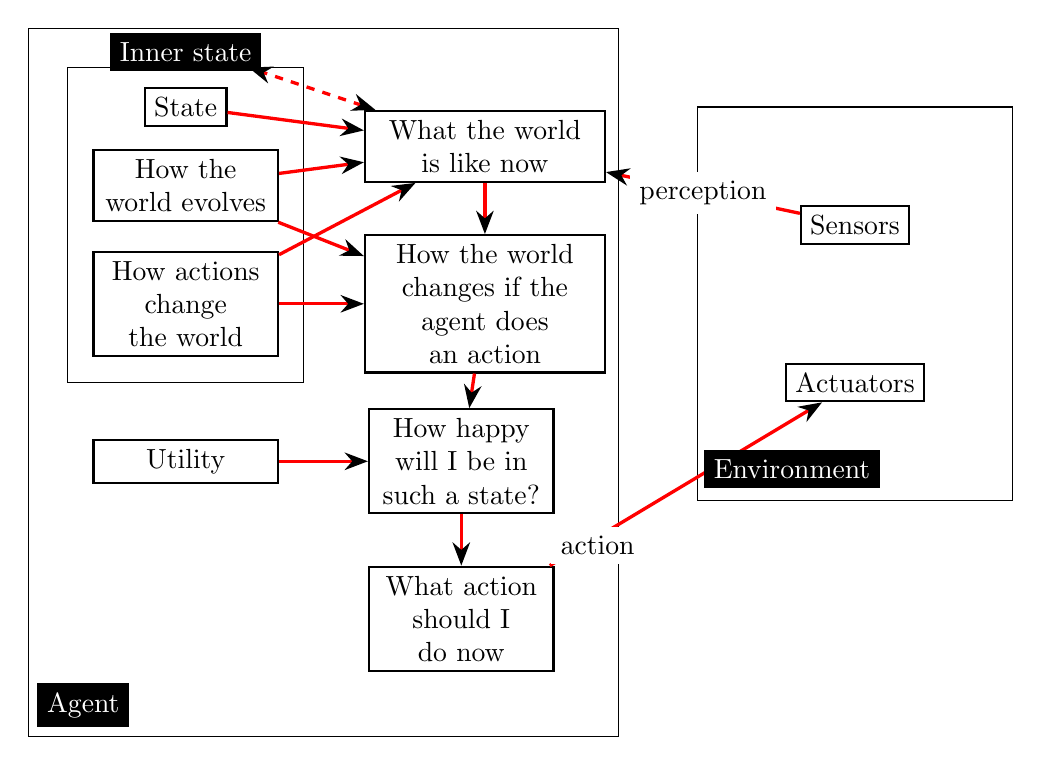
\begin{tikzpicture}

\begin{scope}[every node/.style={circle,thick,draw}]
    % Scene rectangles
    \draw (-2.5,0) rectangle (5,9) [fill=white] {};
    \draw (6,3) rectangle (10,8) [fill=white] {};

    % Inner state
    \draw (-2,4.5) rectangle (1,8.5) [fill=white] {};
    \node (A) at (-0.5,8) [shape=rectangle, fill=white, text centered] 
        {State};
    \node (B) at (-0.5,7) [shape=rectangle, fill=white, text width=6em, text centered] 
        {How the world evolves};
    \node (C) at (-0.5,5.5) [shape=rectangle, fill=white, text width=6em, text centered] 
        {How actions change the world};

    \node (D) at (3.3,7.5) [shape=rectangle, fill=white, text width=8em, text centered] 
        {What the world is like now};

    \node (S) at (3.3,5.5) [shape=rectangle, fill=white, text width=8em, text centered] 
        {How the world changes if the agent does an action};

    \node (E) at (-0.5,3.5)[shape=rectangle, fill=white, text width=6em, text centered] 
        {Utility};

    \node (U) at (3,3.5)[shape=rectangle, fill=white, text width=6em, text centered] 
        {How happy will I be in such a state?};

    \node (F) at (3,1.5)[shape=rectangle, fill=white, text width=6em, text centered] 
        {What action should I do now};

    % Right rectangle - environment
    \node (G) at (8,6.5)[shape=rectangle, fill=white] {Sensors};
    \node (H) at (8,4.5)[shape=rectangle, fill=white] {Actuators};
\end{scope}

\tikzset{CustomEdge/.style={fill=white,rectangle}}

\begin{scope}[>={Stealth[black]},
            %   every node/.style={fill=white,rectangle},
            %   every node/.style={},
              every edge/.style={draw=red,very thick}]
    \path [->] (G) edge node [CustomEdge] {perception} (D);
    \path [<->] (D) edge [dashed] node [] {} (0.3, 8.5);

    % Edges from inner state
    \path [->] (A) edge node [] {} (D);
    \path [->] (B) edge node [] {} (D);
    \path [->] (C) edge node [] {} (D);
    \path [->] (B) edge node [] {} (S);
    \path [->] (C) edge node [] {} (S);

    \path [->] (D) edge [] node [] {} (S);

    \path [->] (S) edge [] node [] {} (U);

    \path [->] (U) edge [] node [] {} (F);

    \path [->] (E) edge [] node [] {} (U);

    \path [->] (F) edge [] node [CustomEdge,above,at start,anchor=south west] {action} (H);
\end{scope}

% \draw (0,1) node [] {Text at \verb!node A!};

\draw (-0.5,8.7) node [rectangle, draw, fill=black, text=white] {Inner state};

\draw (-1.8,0.4) node [rectangle, draw, fill=black, text=white] {Agent};

\draw (7.2,3.4) node [rectangle, draw, fill=black, text=white] {Environment};

\end{tikzpicture}
\end{document}
